\documentclass[12pt]{article}
\usepackage{polski}
\usepackage[utf8]{inputenc}
\usepackage[T1]{fontenc}
\usepackage{amsmath}
\usepackage{amsfonts}
\usepackage{fancyhdr}
\usepackage{lastpage}
\usepackage{multirow}
\usepackage{amssymb}
\usepackage{amsthm}
\usepackage{textcomp}
\frenchspacing
\usepackage{fullpage}
\setlength{\headsep}{30pt}
\setlength{\headheight}{12pt}
%\setlength{\voffset}{-30pt}
%\setlength{\textheight}{730pt}
\pagestyle{myheadings}
%\usepackage{kuvio,amscd,diagrams,dcpic,xymatrix,diagxy}
\usepackage{tikz,paralist,mathtools}
\usetikzlibrary{matrix,arrows,decorations}

\newcommand{\sgn}{{\mathrm{sgn}}\,}
\newcommand{\Kom}{\mathrm{Kom}}
\newcommand{\Mor}{\mathrm{Mor}}
\newcommand{\Hom}{\mathrm{Hom}}
\newcommand{\Ext}{\mathrm{Ext}}
\newcommand{\Ob}{\mathrm{Ob}}
\newcommand{\Cone}{\mathrm{C}}
\newcommand{\Cyl}{\mathrm{Cyl}}
\newcommand{\id}{\mathrm{id}}
\newcommand{\A}{\mathcal{A}}
\newcommand{\B}{\mathcal{B}}
\newcommand{\C}{\mathcal{C}}
\newcommand{\D}{\mathcal{D}}
\newcommand{\Der}{\mathrm{D}}
\newcommand{\Q}{\mathcal{Q}}
\newcommand{\K}{\mathrm{K}}
\newcommand{\qi}{quasi-isomorphism}

\newcommand{\bigslant}[2]{{\left.\raisebox{.2em}{$#1$}\middle/\raisebox{-.2em}{$#2$}\right.}}
\newcommand{\mf}[1]{{\mathfrak{#1}}}
\newcommand{\mb}[1]{{\mathbb{#1}}}
\newcommand{\mc}[1]{{\mathcal{#1}}}
\newcommand{\mr}[1]{{\mathrm{#1}}}


\newcounter{punkt}

\theoremstyle{plain}
\newtheorem{theorem}[punkt]{Theorem}
\newtheorem{lemma}[punkt]{Lemma}
\newtheorem{definition}[punkt]{Definition}
\newtheorem{fact}[punkt]{Fact}
\newtheorem{proposition}[punkt]{Proposition}
\newtheorem{corollary}[punkt]{Corollary}

\theoremstyle{definition}
\newtheorem{remark}[punkt]{Remark}
\newtheorem{example}[punkt]{Example}
\newtheorem{exercise}[punkt]{Exercise}



\markright{Piotr Suwara\hfill Homological algebra II: 29 September 2014\hfill}

\begin{document}

	\begin{remark}
		$\ldots \to \bigslant{\mb Z}{4} \xrightarrow{\cdot 2} 
		\bigslant{\mb Z}{4} \xrightarrow{\cdot 2} 
		\bigslant{\mb Z}{4} \to \ldots$
		is acyclic, so a~$0$ map is a~quasi-isomorphism, but not a~homotopy
		equivalence.
		
		So one has 2 resolutions of $\ldots \to 0 \to \ldots$, which
		are not homotopy equivalent.
	\end{remark}
	
	\begin{definition}[K-injectivity, K-projectivity]
		A~complex $A$ is {\em K-injective (K-projective)} if for any acyclic $X$,
		$\Hom(X,A)$ ($\Hom(A,X)$) is acyclic.
	\end{definition}
	
	\begin{theorem}[Spatenstein]
		In the category of chain complexes of $R$-modules 
		every complex has a~K-injective (K-projective) resolution.
	\end{theorem}
	
	\begin{definition}[$F$-acyclic]
		Assume that $F:\A \to \B$ is left-exact, additive and
		$RF$ ($=\Der^+F$) exists; then we can say that $A \in \A$ is 
		{\em $F$-acyclic}
		if $RF(A)$ has only $0$ cohomology group (i.e. $R^i F(A) = 0$ for $i>0$).
	\end{definition}
	
	\begin{theorem}
		Let $\mc Z$ be a~class of $F$-acyclic objects.
		\begin{itemize}
			\item If $\mc Z$ is sufficiently large,
			then there exists a~class of objects adapted to $F$.
			\item If $\mc Z$ is sufficiently large, 
			then any class of objects adapted to $F$
			is contained in $\mc Z$.
			\item If $\mc Z$ is sufficiently large, 
			then it contains all injective objects of $\A$.
		\end{itemize}
	\end{theorem}
	
	$F: \A \to \B$, $G: \B \to \C$ additive left exact functors
	of abelian categories.
	Assume that there exists classes $\mc{R}_\mc{A}$ of objects adapted to $F$,
	$\mc{R}_\mc{B}$ adapted to $G$, and $F(\mc{R}_\mc{A}) \subset \mc{R}_\mc{B}$.
	These assumptions imply that $RF, RG, R(G \circ F)$ exist.
	
	\begin{theorem}
		The functors $RG \circ RF$ and $R(G \circ F)$
		are isomorphic as functors $\D(\A) \to \D(\C)$.
	\end{theorem}
	
	\begin{remark}
		Assume $X$ is of the type that $R^iF(X)=0$ for $i \neq k$
		for $k$-a~fixed integer.
		Then $RG(RF(X)) = RG(R^kF(X)[-k])$,
		$R^n(G \circ F)(X) = R^{n-k}G(R^kF(X))$.
	\end{remark}
	
	{\bf Triangulated categories}
	
	Assume that $\C$ is an additive category with an automorphism 
	$T:\C \to \C$ (called the {\em translation functor}).
	
	\begin{definition}
		$X[1] = T(X), X[n] = T(X[n-1])$
	\end{definition}
	
	\begin{definition}[triangle]
		A~{\em triangle} in $\C$ is a~sequence of maps
		$X \xrightarrow u Y \xrightarrow v Z \xrightarrow w T(X)$.
		
		A~map of triangles is a~commutative diagram
		
		\begin{tikzpicture}
			\matrix(m)[matrix of math nodes, row sep=1em, column sep=1em]
			{ X & Y & Z & T(X) \\
			  X'& Y'& Z'& T(X') \\};
			\path[->,font=\scriptsize]
			(m-1-1) edge (m-1-2)
			(m-1-2) edge (m-1-3)
			(m-1-3) edge (m-1-4)
			(m-1-1) edge node[auto] {$f$} (m-2-1)
			(m-1-2) edge (m-2-2)
			(m-1-3) edge (m-2-3)
			(m-1-4) edge node[auto] {$T(f)$} (m-2-4)
			(m-2-1) edge (m-2-2)
			(m-2-2) edge (m-2-3)
			(m-2-3) edge (m-2-4);
		\end{tikzpicture}
	\end{definition}
	\pagebreak
	\begin{definition}[triangulated category]
		An additive category $\C$ with $T$ on it is called
		a~{\em triangulated category} if it is equipped
		with a~class of distinguished triangles $(u,v,w)$,
		which satisfy the following conditions:
		\begin{itemize}
			\item TR1. Every morphism $v$ can be embedded into 
			distinguished triangle 
			$X \xrightarrow u Y \xrightarrow v Z \xrightarrow w T(X)$.
			
			Moreover, if $X=Y$ and $Z=0$ and $u=\mr{id}$, then
			$X \xrightarrow{\mr{id}} X \to 0 \to T(X)$
			is distinguished.
			
			\item TR2. $X \xrightarrow u Y \xrightarrow v Z \xrightarrow w T(X)$
			is distinguished iff
			$Y \xrightarrow v Z \xrightarrow w T(X) \xrightarrow{-T(u)} T(U)$
			is distinguished.
			
			\item TR3. Assume that in the diagram
			
			\begin{tikzpicture}
				\matrix(m)[matrix of math nodes, row sep=1em, column sep=1em]
				{ X & Y & Z & T(X) \\
				X'& Y'& Z'& T(X') \\};
				\path[->,font=\scriptsize]
				(m-1-1) edge (m-1-2)
				(m-1-2) edge (m-1-3)
				(m-1-3) edge (m-1-4)
				(m-1-1) edge node[left] {$f$} (m-2-1)
				(m-1-2) edge (m-2-2)
				(m-1-4) edge node[auto] {$T(f)$} (m-2-4)
				(m-2-1) edge (m-2-2)
				(m-2-2) edge (m-2-3)
				(m-2-3) edge (m-2-4);
				\path[->,dotted,font=\scriptsize]
				(m-1-3) edge node[auto] {$h$} (m-2-3);
				\node at (-1.5,0) {$\ast$};
			\end{tikzpicture}
			rows are distinguished and $\ast$ commutes.
			Then there exists $h:Z \to Z'$ such that $(f,g,h)$
			is a~morphism of triangles.
			
			\item TR4. [Octahedron axiom]
			Assume that we have $X,Y,Z,X',Y',Z'$ in $\C$.
			Assume that 
			$X \xrightarrow u Y \xrightarrow j Z' \xrightarrow \partial T(X)$,
			$Y \xrightarrow v Z \xrightarrow x X' \xrightarrow i T(Y)$,
			$X \xrightarrow {v \circ u} Z \xrightarrow y Y' \xrightarrow \delta T(X)$
			are distinguished.
			Then there exists distinguished
			$Z' \xrightarrow f Y' \xrightarrow g X' \xrightarrow {T(j) \circ i} T(Z')$
			such that
			\begin{enumerate}
				\item the four distinguished triangles form faces of octahedron,
				\item the remaining faces commute,
				\item $yv = fj: Y \to Y'$,
				\item $u \delta = i g: Y' \to Y$.
			\end{enumerate}
			
			\begin{tikzpicture}[descr/.style={fill=white}]
				\matrix(m)[matrix of math nodes, row sep=3em, column sep=3em]
				{ & & Z & \\
				Y & X' & & \\
				 & & X & Y' \\
				 & Z' & & \\};
				\path[->,font=\scriptsize]
				(m-2-1) edge node[above] {$v$} (m-1-3)
				(m-1-3) edge node[right] {$y$} (m-3-4)
				(m-1-3) edge node[right] {$x$} (m-2-2)
				(m-2-2) edge node[descr] {$i$} (m-2-1)
				(m-2-1) edge node[left] {$j$} (m-4-2)
				(m-2-2) edge node[descr] {$T(j)\circ i$} (m-4-2);
				\path[->,blue,font=\scriptsize]
				(m-3-3) edge node[right,descr] {$u$} (m-2-1)
				(m-3-3) edge node[descr] {$v \circ u$} (m-1-3)
				(m-3-4) edge node[descr] {$\delta$} (m-3-3)
				(m-4-2) edge node[above left] {$\partial$} (m-3-3);
				\path[->,dashed,font=\scriptsize]
				(m-3-4) edge node[descr] {$g$} (m-2-2)
				(m-4-2) edge node[below] {$f$} (m-3-4);
			\end{tikzpicture}
			\begin{tikzpicture}[descr/.style={fill=white}]
				\matrix(m)[matrix of math nodes, row sep=1em, column sep=1em]
				{ & & & & Z \\
				 & & & & \\
				 & & & & \\
				 & Y & & & \\
				X & & Z & & Y'\\
				 & & & & \\
				 & & & & X'\\};
				\path[->,font=\scriptsize]
				(m-5-1) edge node[auto] {$u$} (m-4-2)
				(m-4-2) edge node[auto] {$j$} (m-1-5)
				(m-5-1) edge node[auto] {$v \circ u$} (m-5-3)
				(m-5-3) edge node[auto] {$y$} (m-5-5)
				(m-4-2) edge node[auto] {$v$} (m-5-3)
				(m-5-3) edge node[auto] {$x$} (m-7-5);
				\path[->,dashed,font=\scriptsize]
				(m-1-5) edge node[auto] {$f$} (m-5-5)
				(m-5-5) edge node[auto] {$g$} (m-7-5);
			\end{tikzpicture}

		\end{itemize}

	\end{definition}


\end{document}
 
 
